\documentclass[12pt, a4paper]{article}
\usepackage[utf8]{inputenc}
\usepackage[polish]{babel}
\usepackage[T1]{fontenc}%polskie znaki
\usepackage[utf8]{inputenc}%polskie znaki

\usepackage{sectsty}
\usepackage{graphicx}
\usepackage{float}
\usepackage{hyperref}

% Margins
\topmargin=-0.45in
\evensidemargin=0in
\oddsidemargin=0in
\textwidth=6.5in
\textheight=9.0in
\headsep=0.25in

\title{ Instrukcja korzystania z serwisu TER}
\author{ Leszek Błażewski\\\\Damian Koper\\\\Karol Noga\\\\Michał Nawrot\\\\Mateusz Wojciechowski}
%\date{\today}

\begin{document}
\maketitle
\pagebreak

% Optional TOC
\tableofcontents
\pagebreak

%--Paper--

\section{Opis i dostępna funkcjonalność narzędzia}

Narzędzie \textit{TER} (z ang. text entities relations) powstało w celu umożliwienia czytelnego zaprezentowania wyników usługi \textit{NER} (z ang. named entity recognition), która pozwala na rozpoznawanie nazw własnych i wyrażeń temporalnych w zadanych przez użytkownika tekstach. Opisywane narzędzie rozszerza serwis NER, między innymi poprzez odpowiednie wyliczanie relacji pomiędzy odnalezionymi bytami na podstawie zadanych wcześniej przez użytkownika parametrów. W kolejnych sekcjach zawarto dostępne w narzędziu funkcjonalności wraz z ich opisami tak aby czytelnik potrafił zrozumieć poszczególne opcje i osiągnąć oczekiwany wynik.

\section{Instrukcja użytkowania}

W poniższym dokumencie opisano wszystkie dostępne funkcjonalności zrealizowanego serwisu wraz z realnym przykładem, gdzie pokazano ich wykorzystanie. Do dokumentu załączono również dwa pliki, dzięki którym każdy czytelnik może śledzić wszystkie modyfikacje na bieżąco i wraz z instrukcją przetestować działanie odpowiednich mechanizmów.

\pagebreak

\subsection{Startowy widok aplikacji}

\begin{figure}[H]
    \centering
    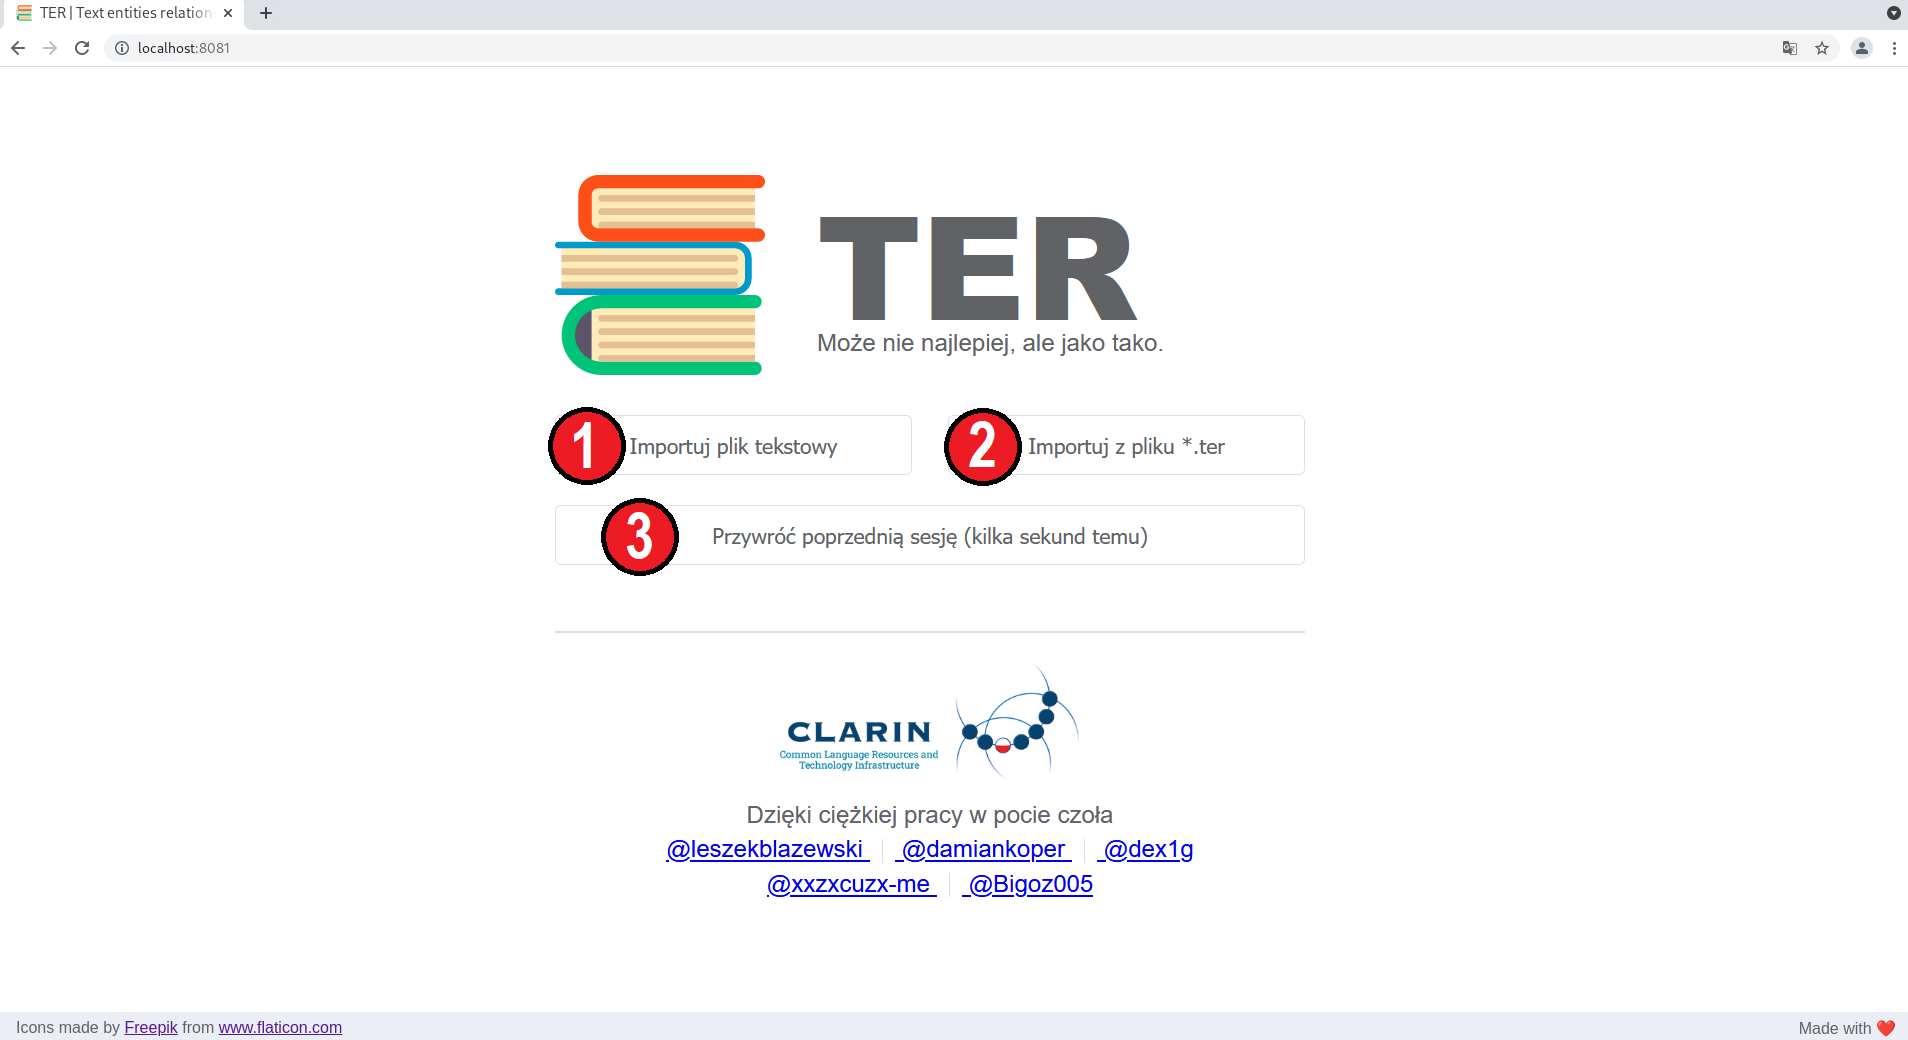
\includegraphics[width=\linewidth]{images/homepage.png}
    \caption{Widok startowy}
\end{figure}

\textbf{Opcja 1, import z pliku} -- Naciskamy przycisk jeśli chcemy wczytać własny tekst i poddać go analizie.\\

\noindent\textbf{Opcja 2, import z pliku ter} -- Wybieramy opcję jeśli posiadamy wygenerowany wcześniej przez aplikację plik o rozszerzeniu \textit{*.ter} lub otrzymaliśmy go od innej osoby. Opcja ta pomija etap analizy tekstu i pozwala bezpośrednio przejść do widoku grafu, który reprezentuje stan wyeksportowany wcześniej z innej sesji w aplikacji. Praca z widokiem grafu została opisana w sekcji \ref{section:graph}.\\

\noindent\textbf{Opcja 3, przewrócenie sesji} -- Jeśli pracowaliśmy już z aplikacją i poddaliśmy jakiś tekst analizie, nasz wcześniej uzyskany stan danych został zapisany i poprzez naciśnięcie przycisku możemy kontynuować pracę od tamtego momentu, przechodząc bezpośrednio na widok grafu. \textit{Uwaga} funkcja ta dostępna jest w zakresie instancji przeglądarki, oznacza to przykładowo, że pracując na przeglądarce Firefox a następnie próbując przywrócić stan w przeglądarce Chrome, zobaczymy, że przycisk będzie niedostępny. Praca z widokiem grafu została opisana w sekcji \ref{section:graph}.

\pagebreak

\subsection{Widok importu plików}

W tej sekcji konfigurujemy wszystkie parametry, które konieczne są podczas analizy importowanego tekstu oraz wykorzystywane są do identyfikacji i modyfikacji relacji pomiędzy odnalezionymi w tekście bytami.

\subsubsection{Dane wejściowe}

\begin{figure}[H]
    \centering
    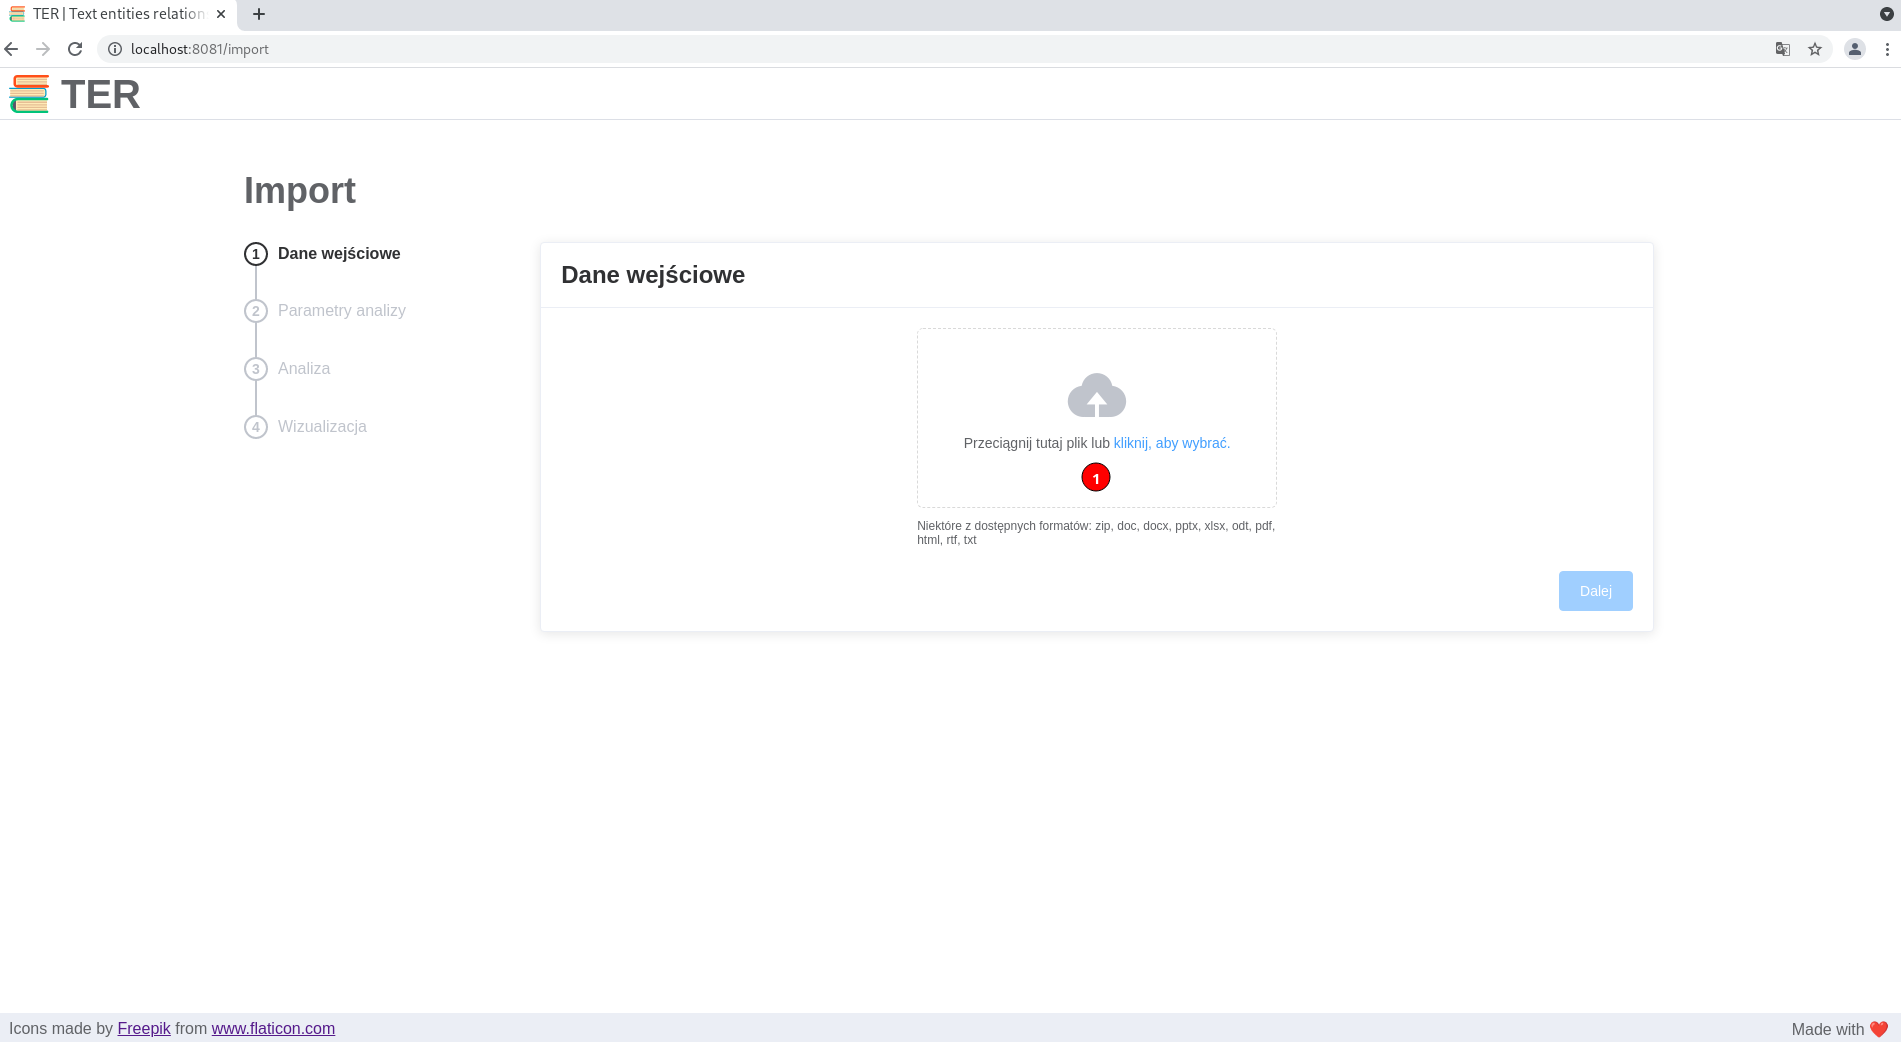
\includegraphics[width=\linewidth]{images/import-before-file.png}
    \caption{Importowanie pliku}
\end{figure}

Po naciśnięciu w zadane miejsce ukaże nam się okno systemowe, gdzie wybieramy plik z tekstem, który następnie poddany zostanie analizie. Plik można również przeciągnąć w wyznaczoną strefę. Jeśli spróbujemy załączyć dwa pliki ukaże nam się następujący komunikat.

\begin{figure}[H]
    \centering
    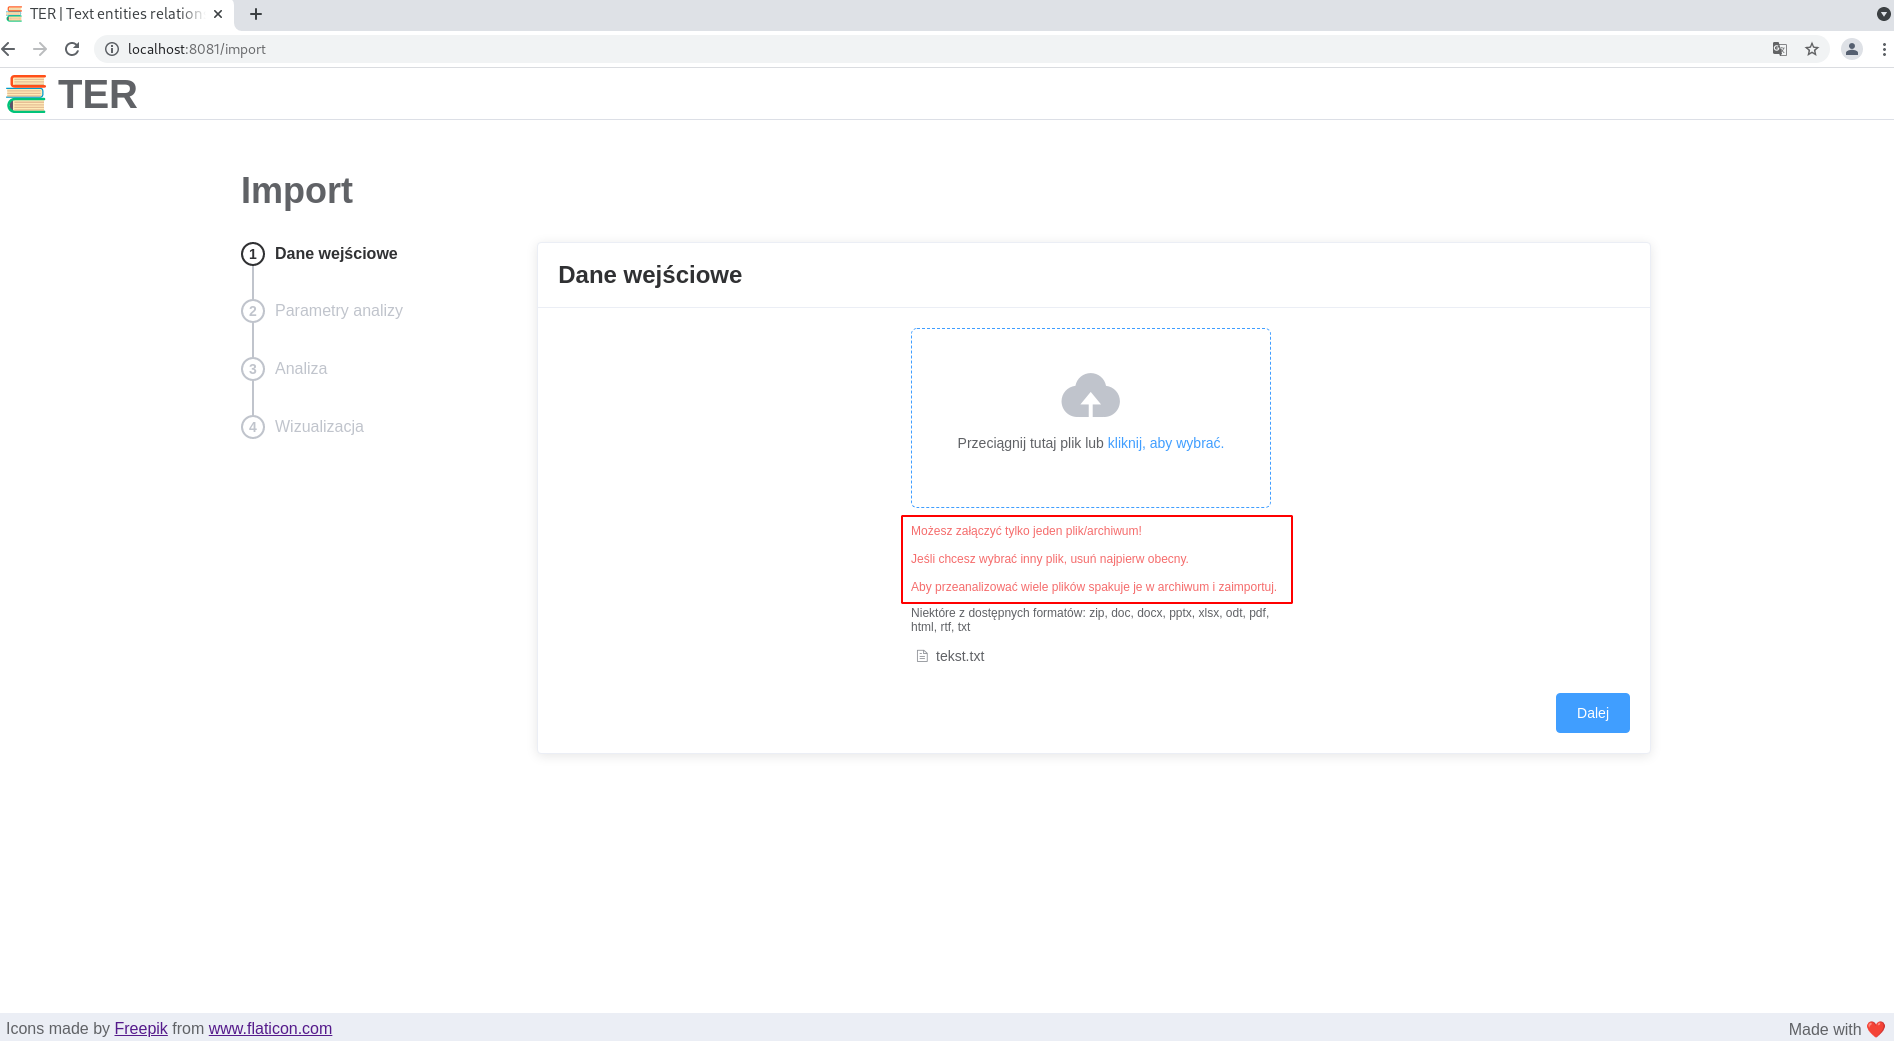
\includegraphics[width=\linewidth]{images/import-error.png}
    \caption{Przekroczenie limitu}
\end{figure}

Zgodnie z informacją załączyć zawsze możemy \textit{jeden} plik lub archiwum. Jeśli chcemy dokonać analizy tekstów, które znajdują się w różnych plikach, należy je wszystkie spakować do archiwum o rozszerzeniu zip i zaimportować uzyskane archiwum do aplikacji. Oczywiście teksty nie muszą być spokrewnione lub pochodzić od jednego autora, narzędzie NER automatycznie dokona ekstrakcji tekstu z przesłanych plików i przeanalizuje dokument jako jedną całość. Dzięki temu możemy przykładowo odnaleźć powiązania między bohaterami z różnych części sagi lub inne analogiczne relacje.

Jeśli popełniliśmy błąd i chcemy wybrać inny plik do zaimportowania, należy najechać na nazwę pliku, który już zaimportowaliśmy (na zrzucie ekranu \textit{tekst.txt}), po czym ukaże nam się krzyżyk po prawej stronie, pozwalający na usunięcie pliku.

Wybierając przycisk \textit{Dalej}, który dostępny jest wyłącznie po wcześniejszym zaimportowaniu pliku/archiwum przechodzimy do ustalenia końcowych parametrów potrzebnych do analizy.

\subsubsection{Parametry analizy}

\begin{figure}[H]
    \centering
    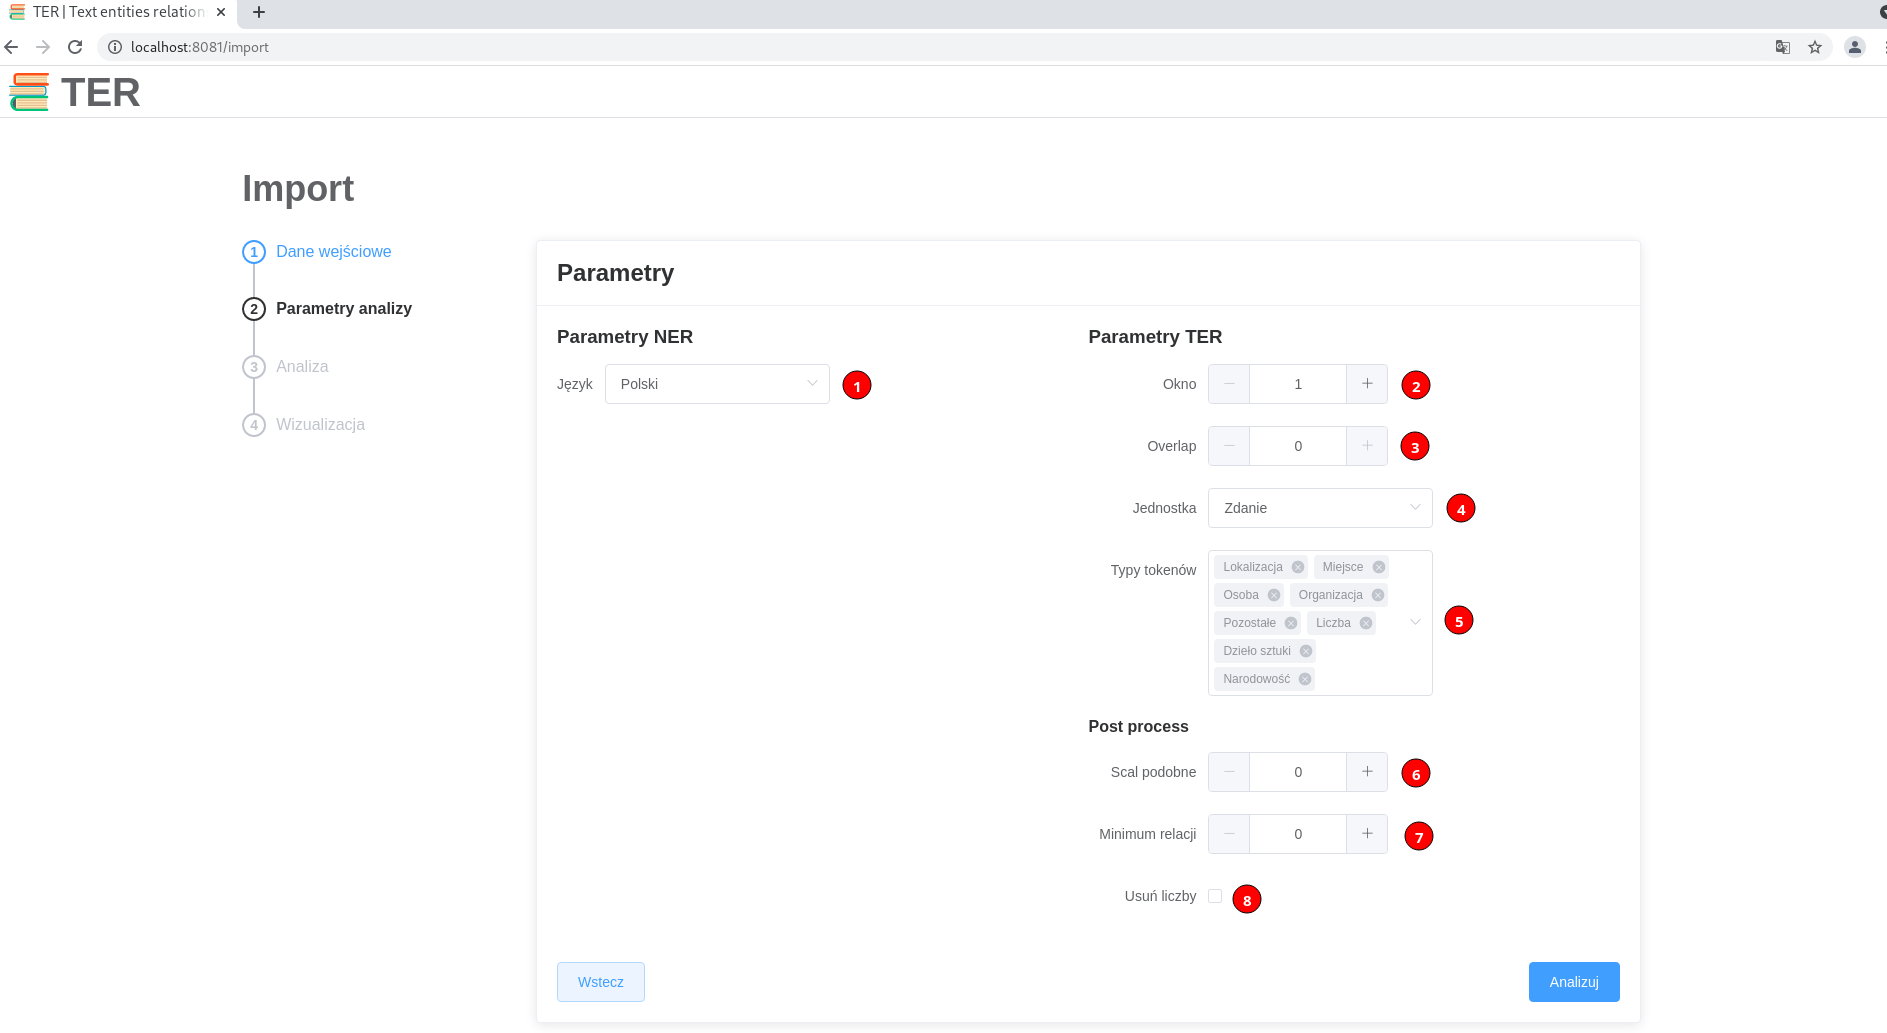
\includegraphics[width=\linewidth]{images/parameters.png}
    \caption{Wybór parametrów analizy}
\end{figure}

\noindent\textbf{Opcja 1, Język} -- Po naciśnięciu na strzałkę ukazuje nam się lista z  obsługiwanymi językami. Wybieramy język w jakim napisany jest zaimportowany wcześniej tekst.\\

\noindent\textbf{Opcja 2, Okno} -- ustalamy wartość okna, czyli zakresu w jakim muszą pojawić się dwa znalezione byty aby algorytm uznał, że są one w relacji. Jak widzimy na zrzucie ekranu w punkcie czwartym w polu jednostka ustawioną mamy wartość zdanie, oznacza to, że okno w zaprezentowanym przykładzie stanowi $1$ zdanie, więc wszystkie słowa, które zostaną zidentyfikowane jako potencjalne byty i \textit{występować będą w obrębie jednego zdania}, zostaną połączone relacją. Jeśli ustawilibyśmy okno na wartość $5$ a w polu jednostka wybralibyśmy wartość paragraf, oznaczałoby to, że wyznaczamy relację spośród wszystkich słów znajdujących się w obrębie $5$ paragrafów w tekście.\\

\noindent\textbf{Opcja 3, Overlap} -- Overlap jest parametrem, który wykorzystywany jest przez algorytm podczas wykrywania relacji miedzy bytami. W zaprezentowanym przykładzie wynosi on $0$ więc oznacza to, że podczas analizy nie wykryjemy żadnych relacji miedzy bytami, które występuję w \textit{różnych} zdaniach(ponieważ jednostka ustawiona jest na wartość \textit{zdanie}, dla pozostałych wartości zachodzi analogiczna sytuacja). Parametr overlap pozwala nam określić ile jednostek(opcja numer 4) ma na siebie nachodzić podczas analizy. Dla przykładu jeśli ustalimy okno na wartość $5$, overlap na $2$ a jednostkę stanowi zdanie, oznacza to iż znalezione byty w obrębie $5$ zdań, gdzie każde kolejne $2$ zdania zazębiają się z poprzednimi będą z sobą w relacji. Tak jak widzimy, parametr pozwala na rozwiązanie problemu analizy bytów wyłącznie w obrębie pojedynczej jednostki wybranej w opcji numer $4$.

\noindent\textbf{Opcja 4, Jednostka} -- Jednostka stanowi wartość, w obrębie, której chcemy wykrywać sąsiedztwo między znalezionymi wcześniej w tekście bytami. Paragrafy rozpoznawane są jako minimum dwa następujące po sobie w tekście znaki nowej linii.\\

\noindent\textbf{Opcja 5, Typy tokenów} -- Narzędzie NER oprócz wykrywania potencjalnych bytów w tekstach, dostarcza również informacji o tym w jaki sposób konkretne słowo zostało zidentyfikowane. Klikając w menu ukaże nam się lista z wszystkimi dostępnymi typami bytów, jeśli nie interesują nas jakieś typy jednostek możemy je tutaj wykluczyć, dzięki czemu zostaną one pominięte podczas wyznaczania sąsiedztwa. Przykładowo w tekście może znajdować się wiele miejsc a nas interesują głównie bohaterowie, więc możemy odznaczyć tą opcję.\\

\noindent\textbf{Opcja 6, Scal podobne} -- Po najechaniu na opcję scalania ukaże nam się komunikat z następującą informacją \textit{Scal wierzchołki, pomiędzy którymi odległość Levenshteina nie przekracza podanej liczby.} Serwis NER nie dokonuje automatycznego połączenia bytów, które w tekście występują w różnych odmianach w związku z czym opcja ta pozwala nam uniknąć wielu encji w końcowym grafie, które w rzeczywistości są na przykład tym samym bohaterem. Łączenie bytów odbywa się na bazie algorytmu Levenshteina, którego opis znaleźć można pod adresem \url{https://pl.wikipedia.org/wiki/Odleg\%C5\%82o\%C5\%9B\%C4\%87_Levenshteina}.\\

\noindent\textbf{Opcja 7, Minimum relacji} -- Po najechaniu na opcję ukaże nam się komunikat z następującą informacją \textit{Usuń wierzchołki, które mają tyle samo lub mniej relacji niż podana liczba.} Jeśli w tekście występuje dużo bytów, które nie wchodzą w relację z innymi, może okazać się, że graf będzie zawierał dużo nieistotnych obiektów, ponieważ przykładowo interesować będą nas tylko główni bohaterowie powieści. Opcja ta pozwala automatycznie pozbyć się bytów, które nie spełniają zadanego minimum, to znaczy, jeśli ilość ich relacji nie jest większa od ustalonej liczby, zostaną one pominięte w końcowym grafie.\\

\noindent\textbf{Opcja 8, Usuń liczby} -- Zaznaczamy opcję jeśli nie chcemy podczas analizy brać pod uwagę byty, które są liczbami. Jest to analogiczna opcja do usunięcia tokenów o typie liczba w opcji numer $5$, lecz narzędzie NER nie zawsze identyfikuje poprawnie rozpoznawane byty w związku z czym opcja ta powinna poprawić końcowy rezultat.\\

Po zakończonej konfiguracji wybieramy przycisk Analizuj, który przeniesie nas na następny widok i automatycznie rozpocznie analizę na podstawie skonfigurowanych parametrów.


\subsubsection{Analiza}

\begin{figure}[H]
    \centering
    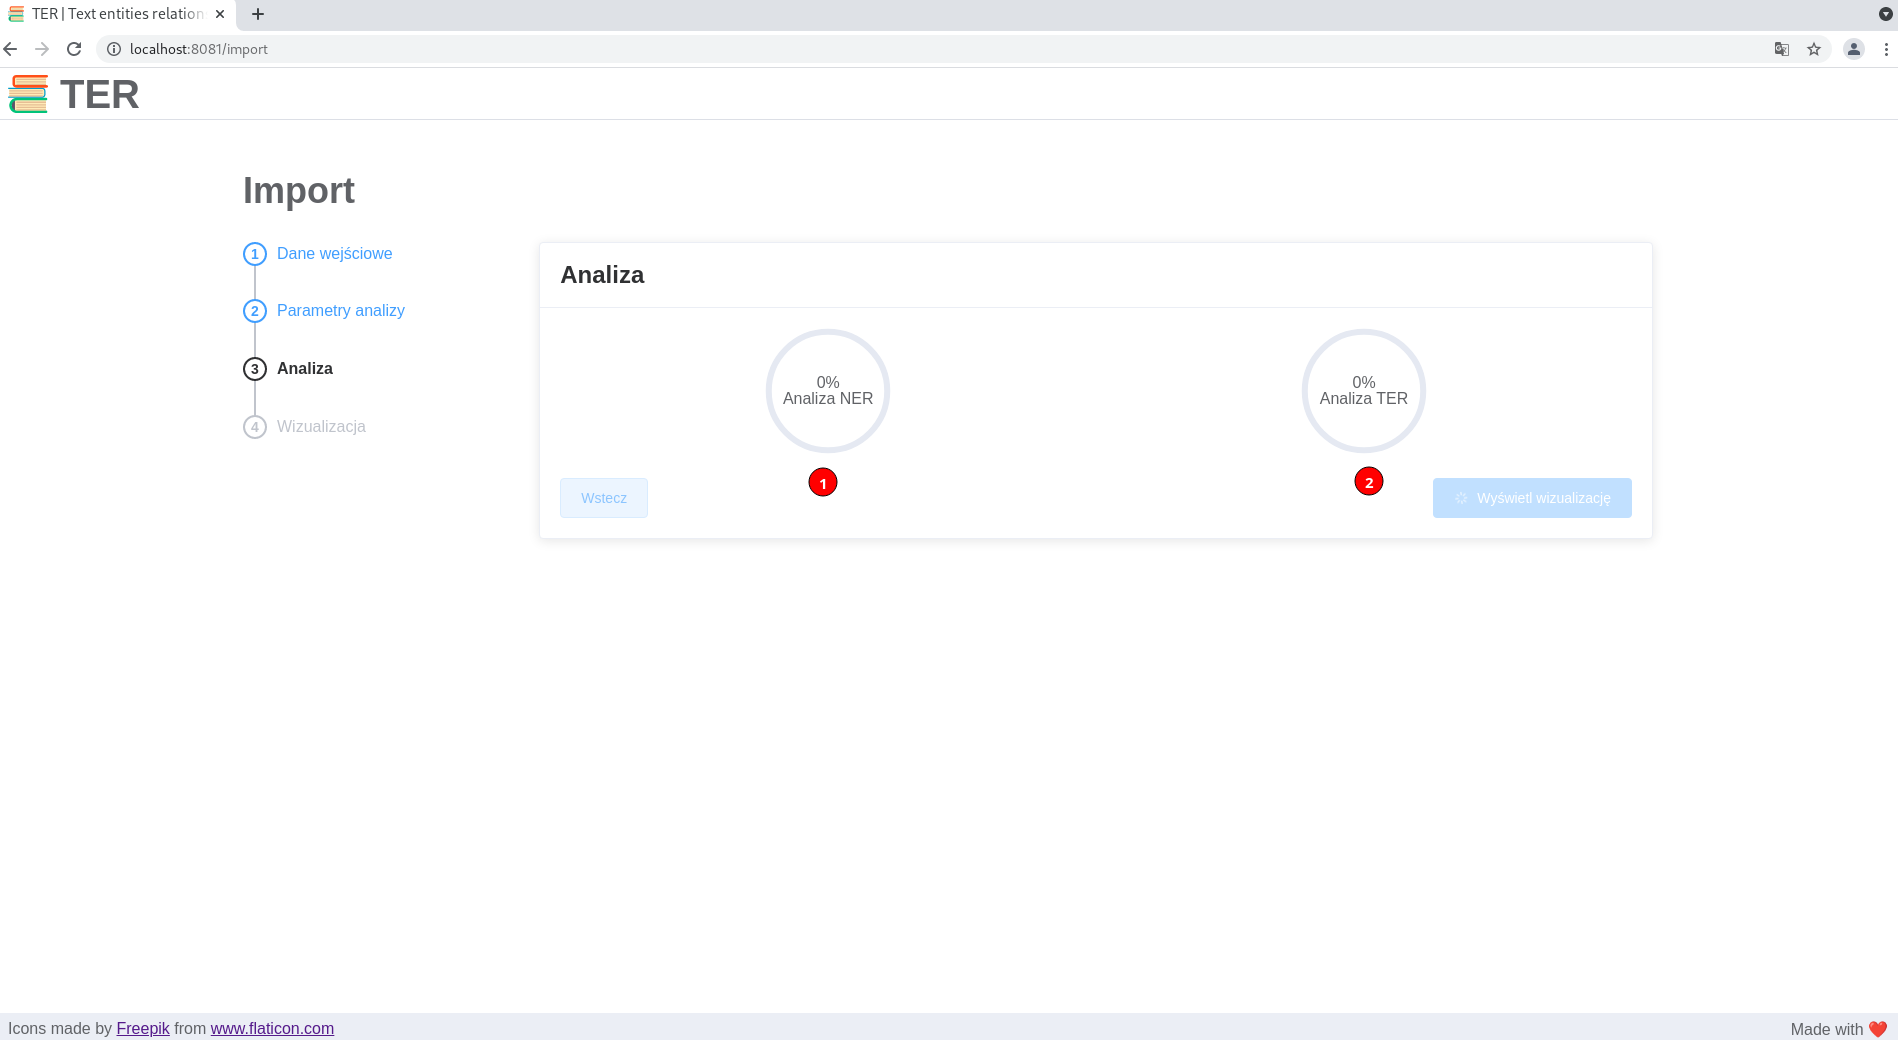
\includegraphics[width=\linewidth]{images/analiza.png}
    \caption{Widok analizy}
\end{figure}

Na tym widoku możemy na bieżąco śledzić postęp analizowanego pliku. Tak długo jak analiza jest w trakcie wykonywania oba przyciski są niedostępne.\\

\noindent\textbf{Postęp 1, Analiza NER} -- Okrąg informuje nas o postępie w analizie pliku przez zewnętrzny serwis NER, który dokonuje wyznaczenie oraz identyfikacji bytów na bazie przekazanych przez nas parametrów. Należy pamiętać, że serwis ten może być wykorzystywany przez wiele osób jednocześnie w związku z czym nasz plik może nie zostać przeanalizowany natychmiastowo i trafi w takim wypadku do kolejki. W takim wypadku nie należy zamykać strony i zaczekać do czasu zakończenia analizy.\\

\noindent\textbf{Postęp 2, Analiza TER} -- Okrąg informuje nas o postępie wykrywania sąsiedztwa pomiędzy zidentyfikowanymi przez serwis NER bytami.

\begin{figure}[H]
    \centering
    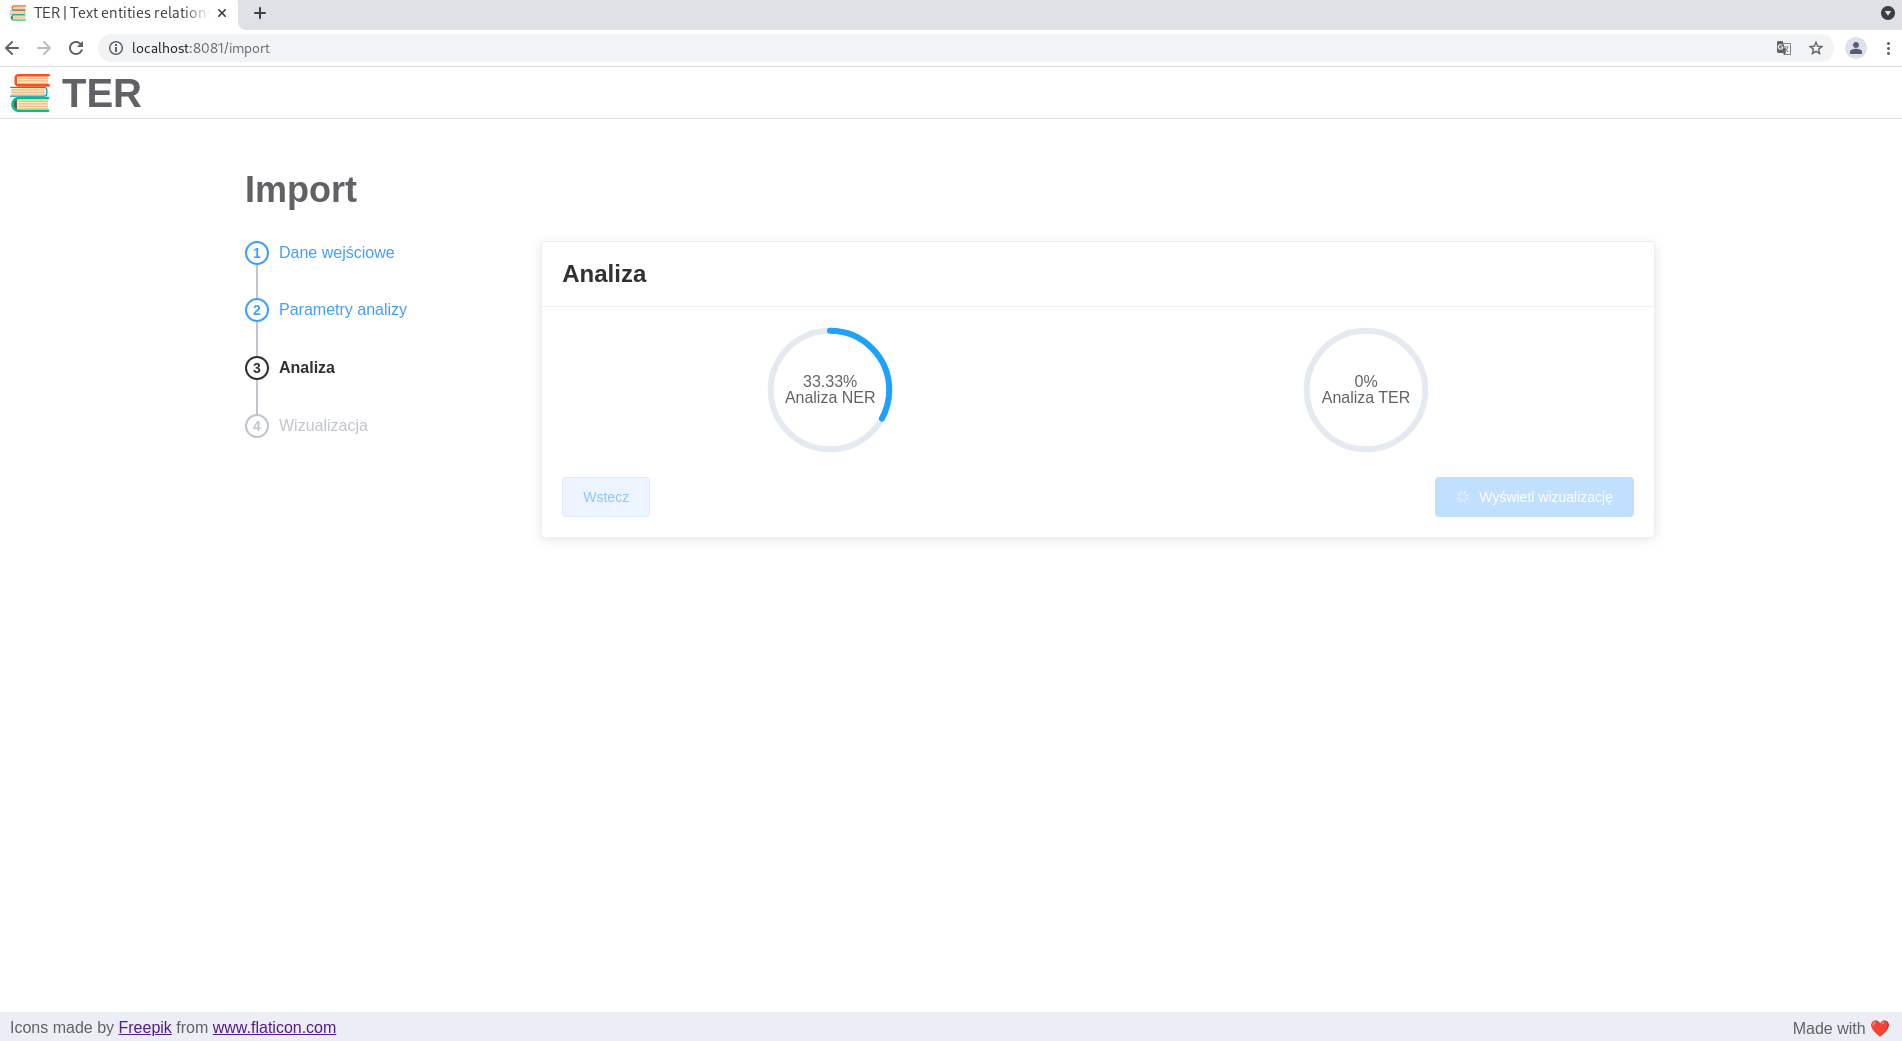
\includegraphics[width=\linewidth]{images/analiza-w-trakcie.png}
    \caption{Postęp w analizie}
\end{figure}

Jeśli podczas analizy dojdzie do błędu, adekwatny komunikat zostanie wyświetlony na ekranie. W takim wypadku, należy skontaktować się z administratorem aplikacji i mieć przygotowany problematyczny plik. Istnieje również możliwość, że serwis NER jest czasowo niedostępny w związku z czym należy spróbować zaimportować plik później.

\begin{figure}[H]
    \centering
    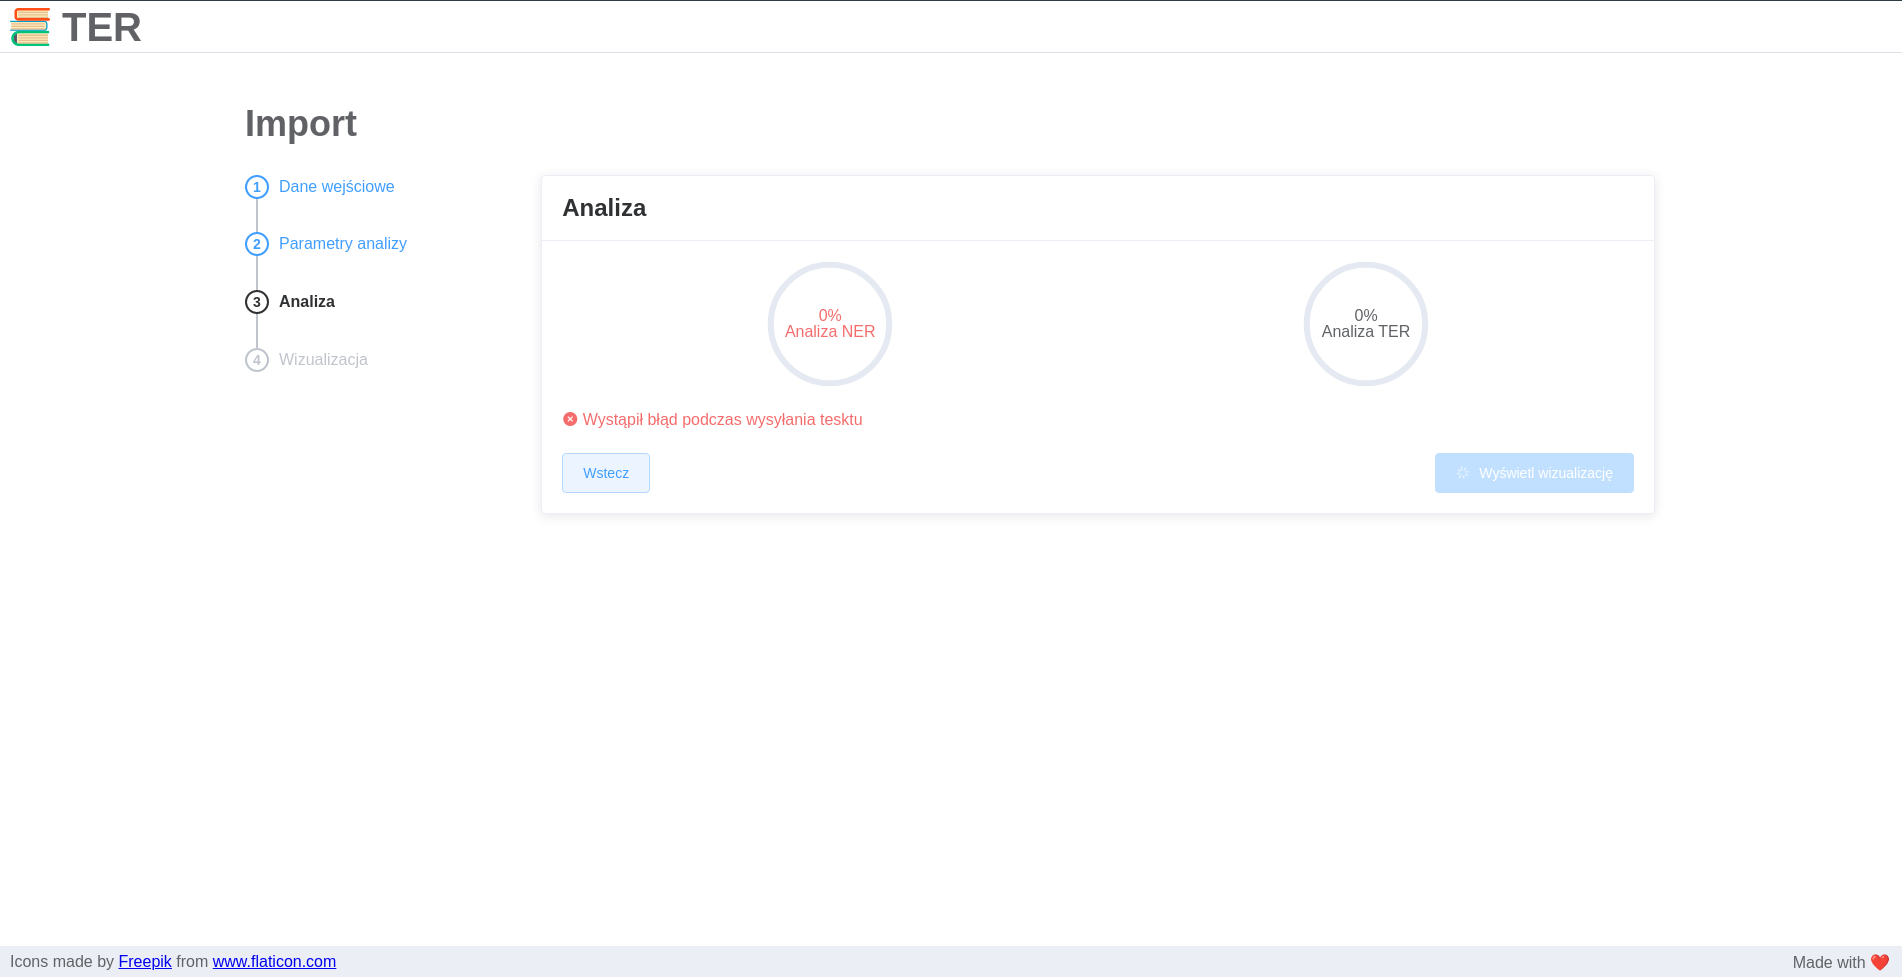
\includegraphics[width=\linewidth]{images/analiza-error.png}
    \caption{Błąd podczas analizy}
\end{figure}

Po poprawnie zakończonej analizie, przy pomocy przycisku wyświetl wizualizację, przechodzi do widoku z grafem, który pozwala nam na interakcję z odnalezionymi bytami.

\begin{figure}[H]
    \centering
    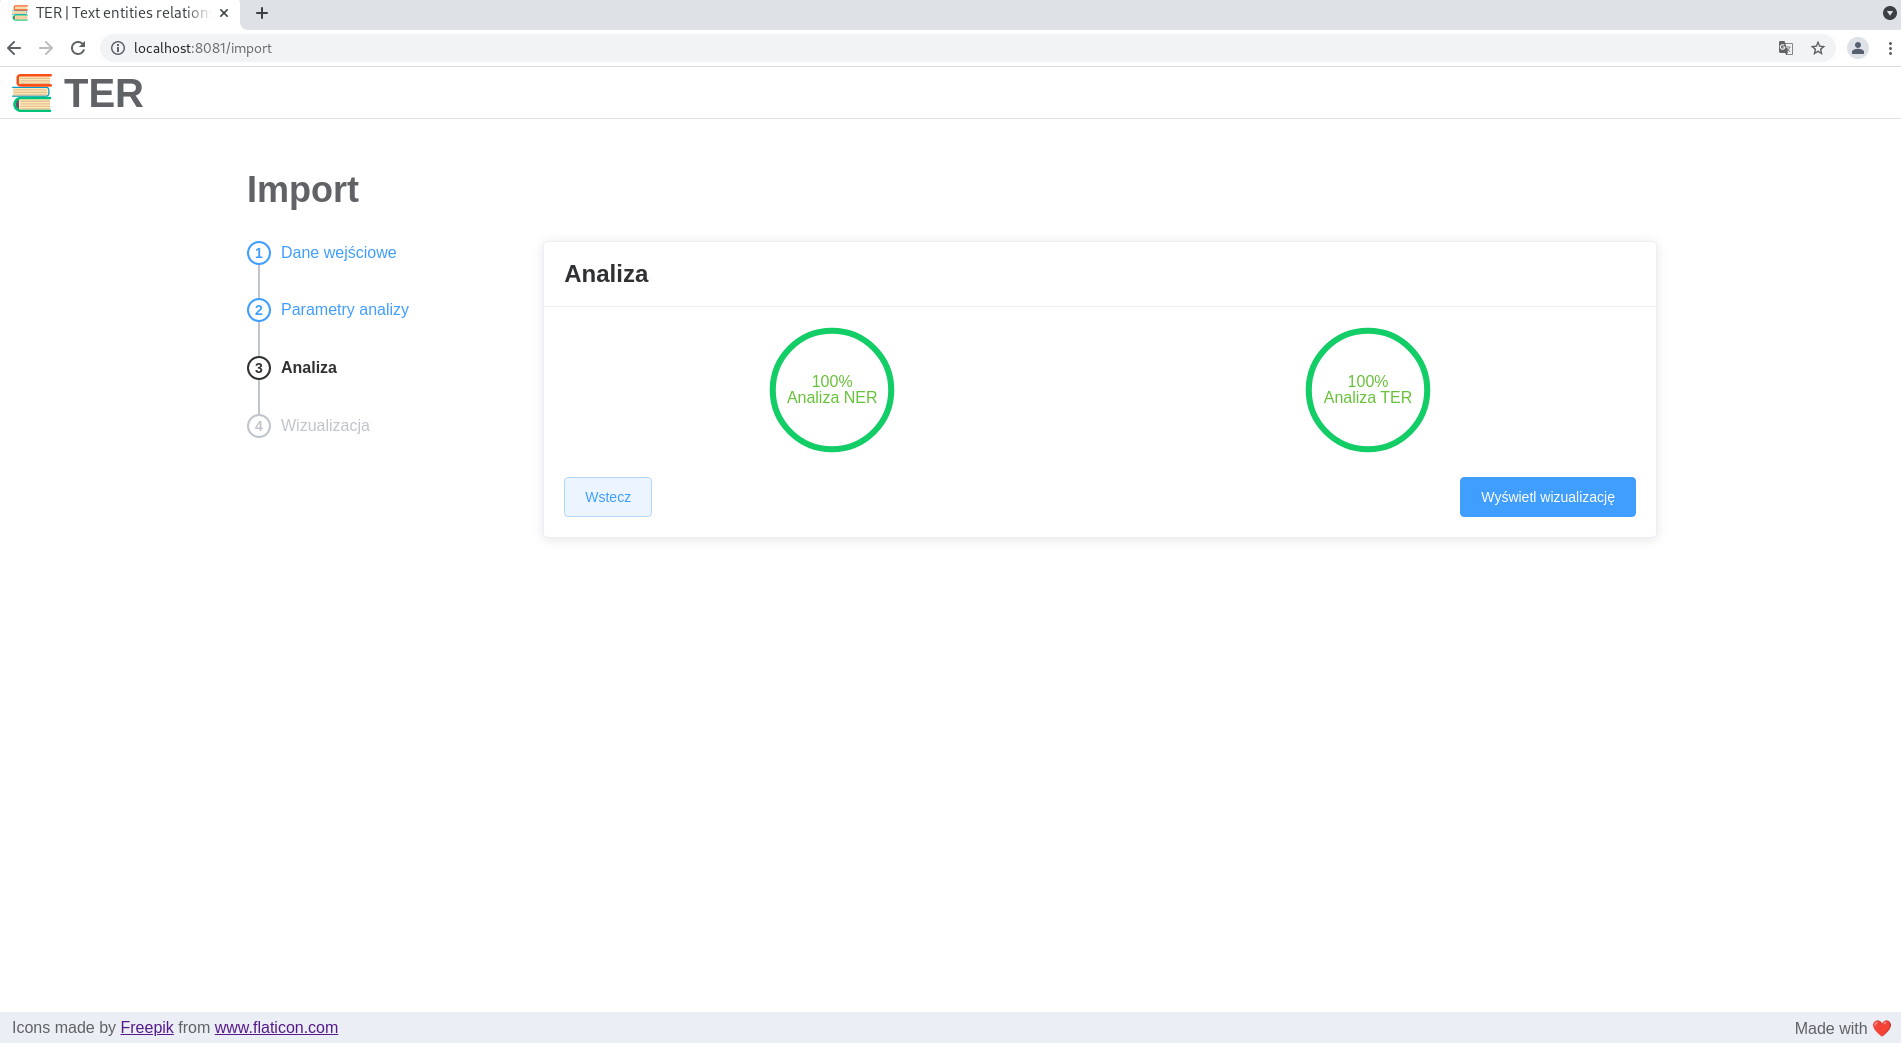
\includegraphics[width=\linewidth]{images/analiza-success.png}
    \caption{Poprawnie zakończona analiza}
\end{figure}


\subsection{Widok grafu prezentującego wizualizację}\label{section:graph}





%--/Paper--

\end{document}